%%
%% This is file `sample-manuscript.tex',
%% generated with the docstrip utility.
%%
%% The original source files were:
%%
%% samples.dtx  (with options: `manuscript')
%% 
%% IMPORTANT NOTICE:
%% 
%% For the copyright see the source file.
%% 
%% Any modified versions of this file must be renamed
%% with new filenames distinct from sample-manuscript.tex.
%% 
%% For distribution of the original source see the terms
%% for copying and modification in the file samples.dtx.
%% 
%% This generated file may be distributed as long as the
%% original source files, as listed above, are part of the
%% same distribution. (The sources need not necessarily be
%% in the same archive or directory.)
%%
%% The first command in your LaTeX source must be the \documentclass command.
%%%% Small single column format, used for CIE, CSUR, DTRAP, JACM, JDIQ, JEA, JERIC, JETC, PACMCGIT, TAAS, TACCESS, TACO, TALG, TALLIP (formerly TALIP), TCPS, TDSCI, TEAC, TECS, TELO, THRI, TIIS, TIOT, TISSEC, TIST, TKDD, TMIS, TOCE, TOCHI, TOCL, TOCS, TOCT, TODAES, TODS, TOIS, TOIT, TOMACS, TOMM (formerly TOMCCAP), TOMPECS, TOMS, TOPC, TOPLAS, TOPS, TOS, TOSEM, TOSN, TQC, TRETS, TSAS, TSC, TSLP, TWEB.
% \documentclass[acmsmall]{acmart}

%%%% Large single column format, used for IMWUT, JOCCH, PACMPL, POMACS, TAP, PACMHCI
% \documentclass[acmlarge,screen]{acmart}

%%%% Large double column format, used for TOG
% \documentclass[acmtog, authorversion]{acmart}

%%%% Generic manuscript mode, required for submission
%%%% and peer review
\documentclass[manuscript,screen,review]{acmart}


%%%
%\usepackage{subfig}
%%%%

%% Fonts used in the template cannot be substituted; margin 
%% adjustments are not allowed.
%%
%% \BibTeX command to typeset BibTeX logo in the docs
\AtBeginDocument{%
  \providecommand\BibTeX{{%
    \normalfont B\kern-0.5em{\scshape i\kern-0.25em b}\kern-0.8em\TeX}}}

%% Rights management information.  This information is sent to you
%% when you complete the rights form.  These commands have SAMPLE
%% values in them; it is your responsibility as an author to replace
%% the commands and values with those provided to you when you
%% complete the rights form.
\setcopyright{acmcopyright}
\copyrightyear{2018}
\acmYear{2018}
\acmDOI{XXXXXXX.XXXXXXX}

%% These commands are for a PROCEEDINGS abstract or paper.
\acmConference[Conference acronym 'XX]{Make sure to enter the correct
  conference title from your rights confirmation email}{June 03--05,
  2018}{Woodstock, NY}
%
%  Uncomment \acmBooktitle if th title of the proceedings is different
%  from ``Proceedings of ...''!
%
\acmBooktitle{Woodstock '18: ACM Symposium on Neural Gaze Detection,
 June 03--05, 2018, Woodstock, NY} 
\acmPrice{15.00}
\acmISBN{978-1-4503-XXXX-X/18/06}

\usepackage{commath,mathtools}
\usepackage{algorithm,algorithmic}
\usepackage{braket,amsfonts,amsopn}
\usepackage{graphicx,subcaption,hyperref,color}
%\usepackage[sort,nocompress]{cite}
\usepackage{tikz}

\usepackage{booktabs}       % professional-quality tables
\usepackage{bm}
\usepackage{multirow}

\newcommand{\ex}{\mathbb{E}}
\newcommand{\pr}{\mathrm{Pr}}
\newcommand{\diag}{\mathrm{diag}}

\DeclareMathOperator*{\argmax}{\mathrm{arg\,max}}
\DeclareMathOperator*{\argmin}{\mathrm{arg\,min}}
\DeclareMathOperator*{\maximize}{maximize}

\newcommand\Fcal{\mathcal{F}}
\newcommand\Rcal{\mathcal{R}}
\newcommand\Ucal{\mathcal{U}}
\newcommand\Xcal{\mathcal{X}}
\newcommand\Abm{\bm{A}}
\newcommand\xbm{\bm{x}}
\newcommand\ebm{\bm{e}}
\newcommand\one{\mathbf{1}}
\newcommand\erm{\mathrm{e}}
\newcommand\trans{^{\top}}
\newcommand{\prob}{\mathbb{P}}
\newcommand{\ebf}{\bm{e}}
\newcommand{\fbf}{\bm{f}}
\newcommand{\gbf}{\bm{g}}
\newcommand{\hbf}{\bm{h}}
\newcommand{\kbf}{\bm{k}}
\newcommand{\mbf}{\bm{m}}
\newcommand{\Mbf}{\bm{M}}
\newcommand{\pbf}{\bm{p}}
\newcommand{\sbf}{\bm{s}}
\newcommand{\ubf}{\bm{u}}
\newcommand{\vbf}{\bm{v}}
\newcommand{\wbf}{\bm{w}}
\newcommand{\xbf}{\bm{x}}
\newcommand{\ybf}{\bm{y}}
\newcommand{\zbf}{\bm{z}}
\newcommand{\qbf}{\bm{q}}

\newcommand{\epsbf}{\bm{\varepsilon}}
\newcommand{\etabf}{\bm{\eta}}
\newcommand{\thetabm}{\bm{\theta}}
\newcommand{\taubf}{\bm{\tau}}
\newcommand{\Kbfbf}{\bm{\Kbf}}
\newcommand{\onebf}{\bm{1}}
\newcommand{\zerobf}{\bm{0}}
\newcommand{\iotabf}{\bm{\iota}}
\newcommand{\phibf}{\bm{\phi}}

\newcommand{\psibf}{\bm{\psi}}
\newcommand{\xibf}{\bm{\xi}}
\newcommand{\gbfbar}{\bar{\bm{g}}}

\newcommand{\fbftd}{\tilde{\bm{f}}}
\newcommand{\fbfbar}{\bar{\bm{f}}}

\newcommand{\Abf}{\bm{A}}
\newcommand{\abf}{\bm{a}}
\newcommand{\Bbf}{\bm{B}}
\newcommand{\Cbf}{\bm{C}}
\newcommand{\Ebf}{\bm{E}}
\newcommand{\Fbf}{\bm{F}}
\newcommand{\Ibf}{\bm{I}}
\newcommand{\Jbf}{\bm{J}}
\newcommand{\Kbf}{\bm{K}}
\newcommand{\Xbf}{\bm{X}}

\newcommand{\chis}{\bm{\chi}_{\mathcal{S}}}
\newcommand{\chisk}{\bm{\chi}_{\mathcal{S}_k}}

% --- mathematical letters
\newcommand{\Gcal}{\mathcal{G}}
\newcommand{\Vcal}{\mathcal{V}}
\newcommand{\Ccal}{\mathcal{C}}
\newcommand{\Dcal}{\mathcal{D}}
\newcommand{\Ecal}{\mathcal{E}}
\newcommand{\Jcal}{\mathcal{J}}
\newcommand{\Lcal}{\mathcal{L}}
\newcommand{\Pcal}{\mathcal{P}}
\newcommand{\Qcal}{\mathcal{Q}}
\newcommand{\Scal}{\mathcal{S}}
\newcommand{\Hcal}{\mathcal{H}}
\newcommand{\Ncal}{\mathcal{N}}

\newcommand{\Ht}{\mathcal{H}(t)}

% --- super/subscripts
\newcommand{\Ipj}{I\cup \{j\}}
\newcommand{\Imi}{I\setminus \{i\}}

\newcommand{\precison}{\text{Prc}}
\newcommand{\recall}{\text{Rcl}}
\newcommand{\accuracy}{\text{Acc}}
\newcommand{\correlation}{\text{Cor}}

\newcommand{\cbm}{\bm{c}}
\newcommand{\gbm}{\bm{g}}
\newcommand{\hbm}{\bm{h}}
\newcommand{\Wbm}{\bm{W}}
\newcommand{\onebm}{\bm{1}}
\newcommand{\phibm}{\bm{\phi}}
\newcommand{\mubm}{\bm{\mu}}
\newcommand{\etabm}{\bm{\eta}}
\newcommand{\zetabm}{\bm{\zeta}}
\newcommand{\Ibm}{\bm{I}}
\newcommand{\lambdabm}{\bm{\lambda}}
\newcommand{\Thetabm}{\bm{\Theta}}
\newcommand{\Sigmabm}{\bm{\Sigma}}
\newcommand{\Psibm}{\bm{\Psi}}
\newcommand{\Gbm}{\bm{G}}
\newcommand{\gammabf}{\bm{\gamma}}
\newcommand{\algrule}[1][.2pt]{\par\vskip.5\baselineskip\hrule height #1\par\vskip.5\baselineskip}


\newcommand{\he}[1]{{\color{blue}{[He: #1]}}}
\newcommand{\red}[1]{{\color{red}{#1}}}

%%
%% Submission ID.
%% Use this when submitting an article to a sponsored event. You'll
%% receive a unique submission ID from the organizers
%% of the event, and this ID should be used as the parameter to this command.
%%\acmSubmissionID{123-A56-BU3}

%%
%% The majority of ACM publications use numbered citations and
%% references.  The command \citestyle{authoryear} switches to the
%% "author year" style.
%%
%% If you are preparing content for an event
%% sponsored by ACM SIGGRAPH, you must use the "author year" style of
%% citations and references.
%% Uncommenting
%% the next command will enable that style.
%%\citestyle{acmauthoryear}

%%
%% end of the preamble, start of the body of the document source.
\begin{document}

%%
%% The "title" command has an optional parameter,
%% allowing the author to define a "short title" to be used in page headers.
\title{Double weighted graph convolutional networks for recommender systems}

%%
%% The "author" command and its associated commands are used to define
%% the authors and their affiliations.
%% Of note is the shared affiliation of the first two authors, and the
%% "authornote" and "authornotemark" commands
%% used to denote shared contribution to the research.
\iffalse
\author{Ben Trovato}
\authornote{Both authors contributed equally to this research.}
\email{trovato@corporation.com}
\orcid{1234-5678-9012}
\author{G.K.M. Tobin}
\authornotemark[1]
\email{webmaster@marysville-ohio.com}
\affiliation{%
  \institution{Institute for Clarity in Documentation}
  \streetaddress{P.O. Box 1212}
  \city{Dublin}
  \state{Ohio}
  \country{USA}
  \postcode{43017-6221}
}
\fi
%%
%% By default, the full list of authors will be used in the page
%% headers. Often, this list is too long, and will overlap
%% other information printed in the page headers. This command allows
%% the author to define a more concise list
%% of authors' names for this purpose.
\renewcommand{\shortauthors}{Trovato and Tobin, et al.}

%%
%% The abstract is a short summary of the work to be presented in the
%% article.
\begin{abstract}
%Graph convolutional networks (GCNs) technique is powerful in learning graph-structured data by integrating node features and topological structure which has been applied on the representation learning in the recommender systems. The GCN-based methods encode both item content information and the historical collaborative signal of user-item interactions to represent items in the embedding space. The user-item interaction information enhanced the performance of representation, but it suffers from cold-start problems since collaborative signals are missing for any new items. 

Graph convolutional networks (GCNs) are very powerful in learning graph-structured data by integrating features from node and its local neighborhood. GCN-based methods can encode features of nodes (items) together with the collaborative signals of user-item interactions to learn the embedding. However, it suffers from cold-start problem as the collaborative signals would be missing for any new nodes. We propose a novel GCN-based representation learning framework for recommender systems by constructing
content and behavioral data into a double connected and weighted hyper-network. Empirical studies on job recommendation scenario shows the effectiveness of our method in representing all nodes in the graph and eliminating the cold-start problem. 
\end{abstract}

%%
%% The code below is generated by the tool at http://dl.acm.org/ccs.cfm.
%% Please copy and paste the code instead of the example below.
%%
\begin{CCSXML}
<ccs2012>
 <concept>
  <concept_id>10010520.10010553.10010562</concept_id>
  <concept_desc>Computer systems organization~Embedded systems</concept_desc>
  <concept_significance>500</concept_significance>
 </concept>
 <concept>
  <concept_id>10010520.10010575.10010755</concept_id>
  <concept_desc>Computer systems organization~Redundancy</concept_desc>
  <concept_significance>300</concept_significance>
 </concept>
 <concept>
  <concept_id>10010520.10010553.10010554</concept_id>
  <concept_desc>Computer systems organization~Robotics</concept_desc>
  <concept_significance>100</concept_significance>
 </concept>
 <concept>
  <concept_id>10003033.10003083.10003095</concept_id>
  <concept_desc>Networks~Network reliability</concept_desc>
  <concept_significance>100</concept_significance>
 </concept>
</ccs2012>
\end{CCSXML}

\ccsdesc[500]{Computer systems organization~Embedded systems}
\ccsdesc[300]{Computer systems organization~Redundancy}
\ccsdesc{Computer systems organization~Robotics}
\ccsdesc[100]{Networks~Network reliability}

%%
%% Keywords. The author(s) should pick words that accurately describe
%% the work being presented. Separate the keywords with commas.
\keywords{graph convolution network, neural networks, embedding, recommender system}

%% A "teaser" image appears between the author and affiliation
%% information and the body of the document, and typically spans the
%% page.
%\begin{teaserfigure}
%  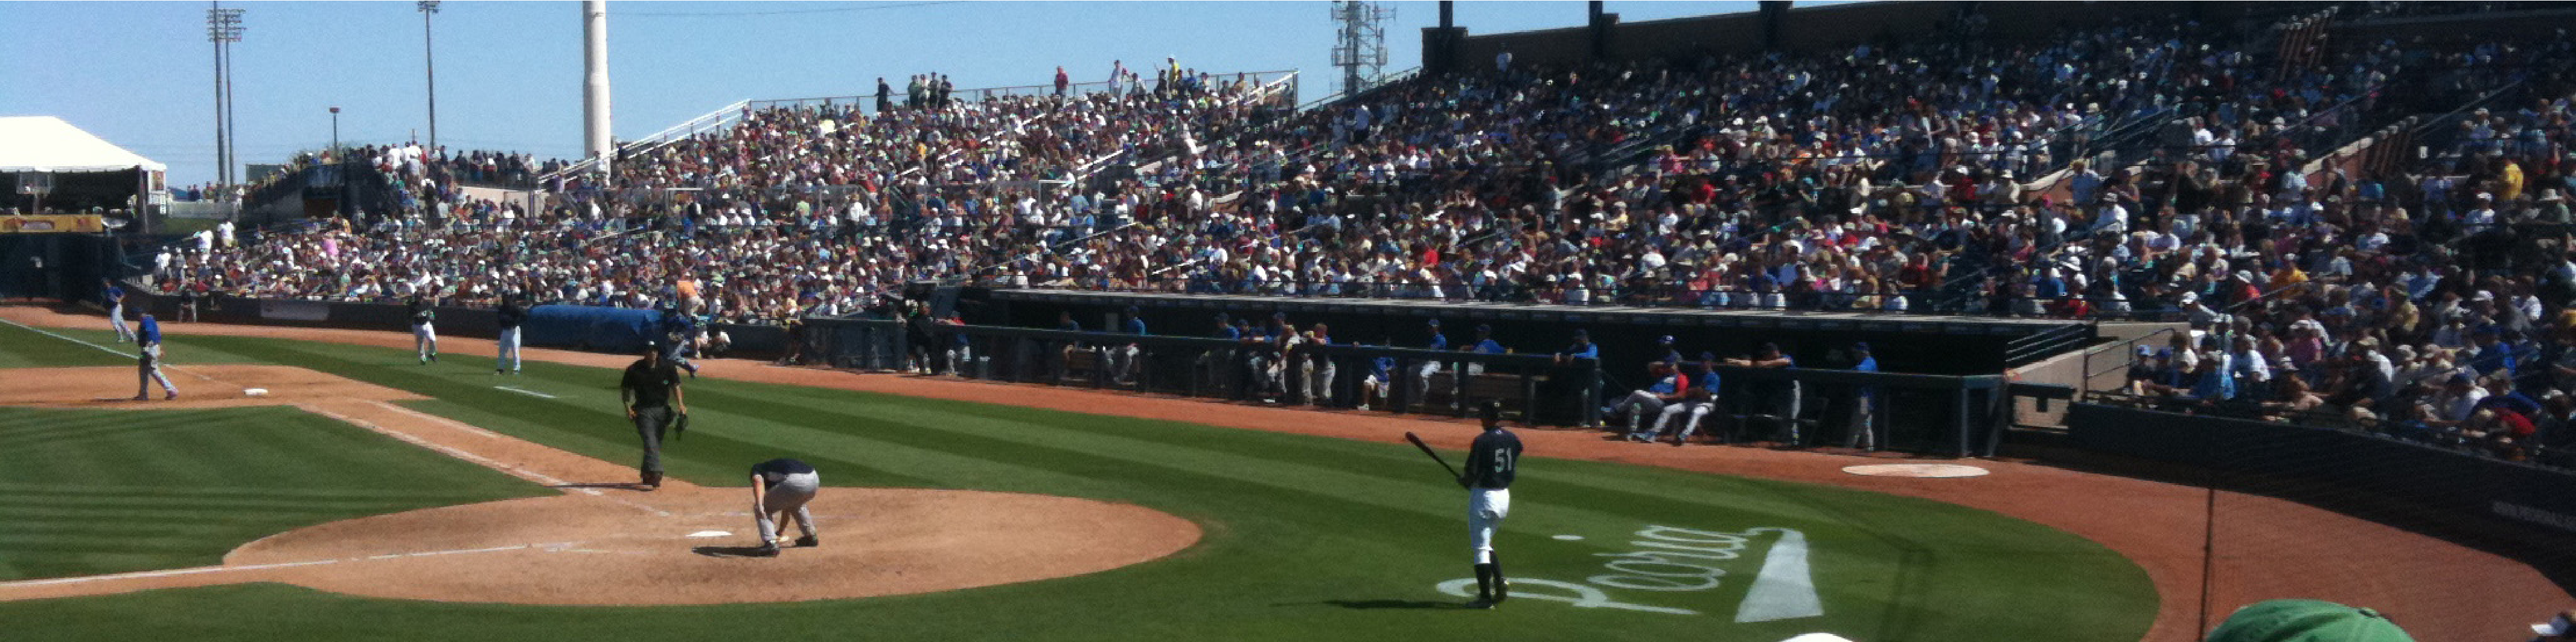
\includegraphics[width=\textwidth]{sampleteaser}
%  \caption{Seattle Mariners at Spring Training, 2010.}
%  \Description{Enjoying the baseball game from the third-base
%  seats. Ichiro Suzuki preparing to bat.}
%  \label{fig:teaser}
%\end{teaserfigure}

%%
%% This command processes the author and affiliation and title
%% information and builds the first part of the formatted document.
\maketitle

\section{Introduction}
% Basic intro to recommender systems and graph structure
Personalised recommender systems have become a crucial component in any online services including e-commerce and job marketplace. The complex relation between users, items and their interactions in online services can be essentially captured in a graph structure. There has been growing interest in leveraging this inherent graph structure for high-level representation of users and items, and applying it to downstream applications such as recommendation.

% Summarize the current state of art on GCN related to recommendation. Clarify what is missing, under what circumstances the current approaches and methods don't work (is insufficient), or have not been explored

Several studies have been done to model and train graph-structured data.  Recently, Graph Convolutional Networks (GCNs) have gained increasing attention and have been shown to be very powerful in representation learning \cite{chen2021structured}. The core idea in Graph Convolutional Networks (GCNs) is to attractively aggregate feature information from local graph neighborhoods by neural networks. GCN-based methods can leverage both content information and graph structure. However, for new items, the association between items to users would be missing, leading to the cold-start problem.

GraphSAGE \cite{hamilton2017inductive} is an inductive deep learning model for graphs that can inference embedding for new nodes without retraining. It uses node feature information to efficiently generate embedding for new nodes. One limitation of this model is that the new nodes should have the same attribute structure as present in the training data. 

%On contrary to our model,  GraphSAGE model is restricted by generating an embeddings for new nodes as long as they have the same attribute structure as the training data. However, our model is free from this limitation.

%State briefly what our proposed solution is, it's strength and how we validate it
With the goal of building an effective (highly relevant) and efficient (near real-time) recommendation system by harnessing graph-structured data,
we propose a novel GCN-based representation learning framework for recommender systems. Our model, referred to as Double Weight Graph Convolutional Neural Network (DWGCN), combines the content and behavioral data in a double connected and weighted hyper-network. We creatively generate a network only based on content, and leverage the user engagement signals to update parameters in model training such that our model can sufficiently benefit from the GCNs, and also eliminates cold-start problem. 

Section \ref{Methodologies}, introduces the preliminaries for our model, and describes the training methodology. In Section \ref{Experiments}, we validate the effectiveness of our method on real-world data for job recommendation in jobs marketplace.


\section{Methodologies} \label{Methodologies}
%\subsection{Problem Definition}

\subsection{Model Description}
\subsubsection{Behavioral and Content based networks}
%As we mentioned, our goal is to get the optimal embeddings for items like jobs. The user engagement network provides supervised connections between similar items, which could be used to measure the quality of the new embedding and also make good parameters updates in the model training. And a graph with connections  defined by the items' content information could help us overcome the cold-start problem on GCN-based methods. 
In this section, we present a novel method to create a Hyper-network (H-network) based on both item content and behavioral information which could be used for a fully GCN-based method. Let $G_{IF}=(V_I\cup V_F,E_c)$ be a bipartite content-based network with two separate parts $V_I$ and $V_F$ where $V_I$ is the set of all items, $V_F$ is the set of all considered filters on items, and $E_c$ is the set of pairs $(i,f)$ such that the item $i\in V_I$ satisfies the filter condition $f\in V_F$. Clearly, while there is a new item, we can easily add it to the network $G_{IF}$. We also consider the engagement network $G_{IU}=(V_I\cup V_U,E_u)$ where $V_U$ is the set of all users and $E_u$ is the set of pairs $(i,u)$ such that user $u$ has some considered interactions with the item $i$. 

Since $G_{IF}$ is bipartite, it identifies a unique multigraph with vertex set $V_I$, edge set $E_I$ such that $i_1i_2\in E_I$ if and only if items $i_1$ and $i_2$ satisfy some common filter, and multiplicity function $\mu: E_I\to \mathbb{N}$ such that $\mu(i_1,i_2)$ is the number of common filters satisfied by items $i_1$ and $i_2$. We denote this multigraph by $G_I=(V_I,E_I,\mu)$. Similarly, the bipartite graph $G_{IU}$ also identifies one unique multigraph $G_I'=(V_I,E_I',\mu')$ where $\mu': E_I'\to\mathbb{N}$ such that $\mu'(i_1,i_2)$ is the number of common user-item interactions of $i_1$ and $i_2$. Finally, we get a behavioral and content based multigraph defined by a 5-tuple $G=(V_I,E_I,E_I',\mu,\mu')$.

\subsubsection{Weighted H-network} To allow the importance of filters and user-item interactions, we could further define a weighted H-network.
Over the multigraph $G_I=(V_I,E_I,\mu)$, let $F:E_I\to \mathcal{F}$ be the filter mapping such that $F(i_1i_2)$ is the set of common passed filters by $i_1$ and $i_2$ where $\mathcal{F}$ is the family of considered filters on items such as required skills, education level, carotene for jobs and so on. Define the weight function $\omega_\mathcal{F}: E_I\to\mathbb{R}$ such that $\omega_\mathcal{F}(i_1i_2)=\sum_{f\in F(i_1i_2)}\omega_f$ where $\omega_f$ is the weight for filter $f$. Note that if $\omega_f=1$ for any $f\in\mathcal{F}$, then $\omega_\mathcal{F}$ is equal to the multiplicity $\mu$. Over the multigraph $G_I'=(V_I,E_I',\mu')$, 
let $\mathcal{C}$ be the family of interactions of users on items (eg. click, application) and $\mu_{\mathcal{C}}=\{multiplicity\ \ \mu_c: c\in\mathcal{C}\}$ be the multiplicity family where $\mu_c: E_I'\to\mathbb{N}$ such that $\mu_c(i_1i_2)$ is the number of common user-item interactions $c$ between $i_1$ and $i_2$. Define the weight function $\omega: E_I'\to\mathbb{R}$ with $\omega(i_1i_2)=\sum_{c\in\mathcal{F}}\omega_c\mu_c$ where $\omega_c$ is the weight for interaction $c$. Finally, we could get two weighted multigraphs $G_I=(V_I,E_I,F,\omega_{\mathcal{F}})$ and $G'_I=(V_I,E_I',\mu_{\mathcal{C}},\omega_{\mathcal{C}})$ for the weighted H-network.

\subsubsection{Sparse weighted H-network} In the item-filter network, we identify the connections between items in $G_I$ in different aspects. We expect the connection are strong enough to show the similarity of items. While $|V_F|<<|V_I|$ in $G_{IF}$, the graph $G_{I}$ will be very dense. To sparse the graph, we could define a hard filter family $\Fcal_h$ to remove weak connections. For example, we could set thresholds $\tau_f$, then modify the graph $G_{I}$ by removing connections between two items with $<\tau_f$ common filters. The hard filters can be also defined by some business logic. For example, we could only consider the items with distance less than a predefined threshold $\tau_l$. The steps to create the sparse weighted H-network are shown in Algorithm~\ref{al:hnet}. 

\begin{algorithm}[h]
\caption{Hyper-network generator}
\begin{algorithmic}[1]\label{al:hnet}
\STATE \textbf{Input:} user engagement network $G_{IU}=(V_I\cup V_U,E_u)$,
item-filter network $G_{IF}=(V_I\cup V_F,E_c)$, 
hard filter family $\mathcal{F}_h$,
Filter family $\mathcal{F}$ with weights $\{\omega_f:f\in\mathcal{F}\}$,
interaction family $\mathcal{C}$ with weights $\{\omega_c:c\in\mathcal{C}\}$
%\STATE \textbf{Initialization:} $\ubf\in \Ucal$.
\STATE \textbf{Step 1.} find a maximal matching $M_f$ and $M_u$ on $G_{IU}$ and $G_{IF}$, respectively.
\STATE \textbf{Step 2.} do edge contractions on graph $G_{IF}$ and $G_{IU}$ over edges in $M_f$ and $M_u$, respectively. Denote the result multigraphs as $G_I=(V_I,E_I,F,\omega_{\mathcal{F}})$ and $G'_I=(V_I,E_I',\mu_{\mathcal{C}},\omega_{\mathcal{C}})$.
\STATE \textbf{Step 3.} Remove job connections by hard filters in $\mathcal{F}_h$, update $E_I$.
\STATE 
\textbf{Output:} H-network $G=(V_I,E_I\cup E_I',\omega_{\mathcal{F}},\omega_{\mathcal{C}})$.
\end{algorithmic}
\end{algorithm}

\subsubsection{Neighbor importance selection} 
GCNs is a neighborhood aggregation scheme, but the size of node neighborhoods are irregular in the H-network. In order to keep the computational footprint in the training, we convolve on node over its selected  neighborhood of fixed size. Moreover, in the H-network, both $\omega_{\Fcal}$ and $\omega_{\Ccal}$ measure the strength of connections. Stronger the connection, more reliable the neighbor information is going to be.
However, we note that $\omega_{\Ccal}$ is missing for new items.
To avoid cold-start problem, we only use $\omega_{\Fcal}$ in the GCNs to weight the importance of neighbors.
Thus, we define a neighbor importance selection function $\Ncal^*: V^I\times\mathbb{N}\to V^I$ to generate the neighborhood for nodes such that $\Ncal^*(v,k)$ is a set of neighbors of node $v$ with size $k$ which are randomly selected by weights $\omega_{\Fcal}$.
Note that, we only select neighbors related to edges in $E_I$.  For notation simplicity, let $\Ncal^{(k)}_v$ be the selected $k$-hop neighborhood of node $v$ and $\Ncal_v$ be the whole neighborhood defined by the filter edge set $E_I$. Given neighborhood sizes $k$,  if $|\Ncal_v|< k$, then the neighbors of $v$ are sampled with replacement in $\Ncal^*(v,k)$. 
More details are shown in Algorithm~\ref{alg:nodes}. 

\begin{algorithm}[h]
\caption{Neighborhood importance selection on node $u$}
\label{alg:nodes}
\begin{algorithmic}[1]
\STATE \textbf{Input:} Node $u$, filter edge set $E_I$, filter weight function $\omega_{\Fcal}$, depth $K$, neighborhood sizes $s_k$ for $k=1,2,\cdots,K$.
\STATE \textbf{Initialization:} $\Ncal_u^{(0)}:=\{u\}$ and $\Ncal_u^{(k)}:=\emptyset$ for $k=1,2,\cdots,K$.
\FOR{ $k=1,\cdots,K$}
\FOR{$v\in \Ncal_u^{(k-1)}$}
\STATE $N\leftarrow$ Randomly selected $s_k$ neighbors from $\Ncal_v:=\{w: vw\in E_I\}$ by weights $\{\omega_{\Fcal}(vw): w\in\Ncal_v\}$ with replacement if $|\Ncal_v|<s_k$, and without replacement otherwise.
\STATE $\Ncal_u^{(k)}\leftarrow \Ncal_u^{(k)}\cup N$
\ENDFOR
\ENDFOR
\STATE 
\textbf{Output:} $k$-hoop neighborhood $\Ncal_u^{(k)}$ for $k=1,2,\cdots,K$.
\end{algorithmic}
\end{algorithm}

\subsubsection{Model Architecture}
As in all GCN-based methods, the core of our DWGCN algorithm is to use the localized convolutional modules to generate embeddings for nodes. It starts with node features and its localized graph structures in the H-network, and then learn the GCNs that transform and aggregate features of the node neighborhood. If there are some node features given as text descriptions, then we should be embedding them as numerical vectors by some general or pre-trained text to vector embedding models. The rough text embedding combined with other numerical features are called the current embedding for nodes. Let $c_u$ be a current embedding for node $u\in V_I$, then the task is to generate a new embedding $n_u$ to optimally identify the node's features. The procedure is detailed in Algorithm~\ref{alg:gcns}.

\begin{algorithm}[h]
\caption{Node neighborhood aggregator on node $u$}
\label{alg:gcns}
\begin{algorithmic}[1]
\STATE \textbf{Input:} H-network $G=(V_I,E_I\cup E_I',\omega_{\mathcal{F}},\omega_{\mathcal{C}})$, current embedding set $\{c_v: v\in V_I\}$, activation function $\sigma(\cdot)$, depth $K$, $k$-hoop neighborhood $\Ncal_u^{(k)}$,weights $\mathbf{W^{(k)}}$, biases $\mathbf{b}^{(k)}$, aggregator functions $g^{(k)}$ for $k=1,2,\cdots,K$.
\STATE \textbf{Initialization:} $h_v^{(K)}:=c_v$ for $v\in \Ncal_u^{(K)}$ and $\Ncal_u^{(0)}:=\{u\}$.
\FOR{ $k=K,\cdots,1$}
\FOR{ $z\in \Ncal^{(k-1)}_u$}
\STATE \it{Convolve over neighborhood}: $h_z^{(k-1)}\leftarrow g^{(k)}\left(\{h^{(k)}_v: \forall{v}\in \Ncal_z\cap \Ncal^{(k)}_u\}\right)$
\STATE \it{Convolve with self-embedding:} $h_z^{(k-1)}\leftarrow \sigma\left(\mathbf{W}^{(k)}\cdot CONCAT(h_z^{(k-1)},c_z)+\mathbf{b}^{(k)}\right)$.
\STATE \it{Normalization: }
$h_z^{(k-1)}\leftarrow h_z^{(k-1)}/||h_z^{(k-1)}||_2$.
\ENDFOR
\ENDFOR
\STATE 
\textbf{Output:} New embedding $n_u:=h_u^{(0)}$ for node $u$.
\end{algorithmic}
\end{algorithm}



\subsection{Model Training}
\subsubsection{Weighted Energy-based Loss Function} We train the DWGCN in a fully unsupervised manner which assumes that two connected nodes in the H-network have more similar representations than non-connected node pairs. In particular, for any edges $uv, uw\in E_I\cup E_I'$, if $\omega_{\Fcal}(uv)+\omega_{\Ccal}(uv)> \omega_{\Fcal}(uw)+\omega_{\Ccal}(uw)$, then we have $n_u\cdot n_v> n_u\cdot n_w$. Note that, differ from the step for neighborhood sampling which only consider filter edges in $E_I$, the customer behavioral edge set $E_I'$ is also considered here. Since the user-item interaction information is only used to teach the model on the reliable connections in the backward step, the algorithm is designed for applications which fully overcome the cold-start problem.
% \vspace*{-5mm}
Define the weight $\omega_{u_1u_2}:=0.5*\left(\omega_{\Fcal}(u_1u_2)+\omega_{\Ccal}(u_1u_2)\right)$ for $u_1u_2\in E_I\cup E_I'$, and $\omega_{u_1u_2}:=0$ otherwise.
For an edge $uv\in E_I\cup E_I'$, consider the weighted loss function for their node embeddings $n_u,n_v$ 
\[\mathcal{L}(n_u,n_v)=-\omega_{uv}\log\left(\sigma(n_u\cdot n_v)\right)-N*\mathbb{E}_{w\sim P_u}(1-\omega_{uw})\log\left(\sigma(-n_u\cdot n_w)\right)\]
where $P_u$ denotes the distribution of negative samples for item $u$, $N$ is the number of negative samples, and $\sigma(\cdot)$ is the sigmoid function. It introduces weights on the cost of missing a positive or negative sample.


\subsubsection{Strategy on negative sampling.} 
To enforce the model to learn the parameters to capture the difference of strong and weak connections, instead of uniformly sample negative instances from the entire set of nodes we consider the connections with small weights as the hard negative samples. 

\section{Experiments} \label{Experiments}
We test and evaluate the new embedding generated by our proposed system with a real dataset via CareerBuilder.com
on the related job recommendation task. The objective is to find jobs a user might be interested in. To capture user's interests,
we take one of the most recently applied jobs by the user as source job, then find the closest jobs in the new embedding space to the source for recommendation. In the experiment, the top 100 closest jobs are selected.

In the implementation, we generate the user engagement network with the users' job application behavior, and the job-filter network with filters related to job title, carotene, location, and so on. More specifically, for job $j$ and user $u$, if $u$ applied job $j$ after posted, then the connection $(u,j)$ is generated in the user engagement network $G_{IU}$. By Algorithm~\ref{al:hnet}, if there is a user $u$ applied both job $j_1$ and $j_2$, then $j_1j_2\in E_I'$ and its weight $\omega_{\Ccal}(j_1j_2)$ is measured by the co-apply counts (co-apps).  For the multigraph $G_I$ generated from the job-filter network $G_{IF}$, we consider connections for jobs $j_1,j_2$ with the same posted job title, same normalized job title, same carotene, same the first four digits of carotene, same requested skills, or sim-score $\geq0.9$. The sim-score is the cosine similarity score of current embeddings. For connection $j_1j_2$ in $G_I$, we define the weight $\omega_{\Fcal}$ by an aggregated scores on filter scores and location distance that the parameters are decided by the parameter tuning.  We normalize both $\omega_{\Fcal}$ and $\omega_{\Ccal}$, then use $\omega_{\Fcal}(uv)+\omega_{\Ccal}(uv)<1$ for $uv\in E_I\cup E_I'$ as hard filter to filter out weak connections.
Finally, we are ready to generate the H-network $G=(V_I,E_I\cup E_I',\omega_{\mathcal{F}},\omega_{\mathcal{C}})$ by Algorithm~\ref{al:hnet}.

%\subsubsection{Data preparation}
Since the DWGCN can efficiently represent unseen nodes in the network, we only train the model in a subgraph. To evaluate the performance of new embeddings by the users' application behaviors, we only consider nodes covered by enough co-apply edges. Thus    
over the user engagement network, we select the subgraph reduced by connections with co-apps$\geq20$.
Moreover, in the training, the jobs modified by the system during 12/01-12/06 are used. When testing we run the inference on the entire subgraph with jobs modified by the system during 12/01-12/09 to generate embedding for all jobs, and the jobs modified in 12/07-12/09 are used to test the recommendation performance. Note that we suppose all test jobs are new jobs without any apply signals detected, so only content-based connections are used for test jobs.
Overall we use 615,000 pairs of positive training examples and 20 negative examples per node. 

%\subsubsection{Features used for learning and baselines}
The current 150-dimensional job embeddings by DLEM~\cite{zhao:2021embedding} concatenated with the 3-dimensional Cartesian coordinates transformed from the spherical coordinates of latitude and longitude are used as features. We also evaluate the performance of DWGCN against DLEM~\cite{zhao:2021embedding}  which is the  state-of-the-art content-based method to embed job description, title to numerical vectors by multiple neural networks. Furthermore, we conduct ablation studies and consider several variants of aggregator functions defined in \cite{hamilton2017inductive} for DWGCN: Mean, Meanpooling and GCN. For all the variants, we set the depth $K=2$, sample sizes $s_1=25,s_2=10$, and the hidden and output dimensions to be both 128.
Table~\ref{tab:comp} shows the results of the head-to-head comparison between DWGCN compiled with three different aggregator functions and the baseline DLEM~\cite{zhao:2021embedding} on the co-apps where the method wins the DLEM for a source job $j$ if there are more co-apps on job $j$ and its recommended jobs. It indicates that the embeddings generated by DWGCN is outperformed than DLEM to find related jobs and capture user's interests.  

\begin{table}[t]
  \caption{Head-to-head comparison on relevancy of source job and recommended jobs by co-apps counts}
  \label{tab:comp}
  \begin{tabular}{lcccccccccc}
    \toprule
    Methods & Win & Lose & Draw \\
    \midrule
    DWGCN-Mean vs. DLEM& \textbf{54.64\%} & 29.96\% & 15.40\%\\
    DWGCN-Meanpooling vs. DLEM& \textbf{48.80\%} & 35.51\% & 15.68\%\\
    DWGCN-GCN vs. DLEM & \textbf{61.49\%} & 15.77\% & 22.75\%\\
  \bottomrule
\end{tabular}
\end{table}
 

\section{Conclusion and future work}
We proposed a GCN-based approach to encode item features and user-item interaction information into the graph structure to represent items. The new embeddings are able to capture content features of items, and also the behavioral information of users on the related items. Moreover, it can fully overcome cold-start problem. In this work, we only discussed the representation learning for items, but the framework can be easily extended to representation learning on users, or on users and items in the shared space. 

%%
%% The acknowledgments section is defined using the "acks" environment
%% (and NOT an unnumbered section). This ensures the proper
%% identification of the section in the article metadata, and the
%% consistent spelling of the heading.
% \begin{acks}
% To Robert, for the bagels and explaining CMYK and color spaces.
% \end{acks}

%%
%% The next two lines define the bibliography style to be used, and
%% the bibliography file.
\bibliographystyle{ACM-Reference-Format}
\bibliography{refs}

%%
%% If your work has an appendix, this is the place to put it.
\appendix


\end{document}
\endinput
%%
%% End of file `sample-authordraft.tex'.
